\documentclass[lettersize,journal]{IEEEtran}
\usepackage{amsmath,amsfonts}
\usepackage{hyperref}
\usepackage{algorithmic}
\usepackage{algorithm}
\usepackage{array}
\usepackage[caption=false,font=normalsize,labelfont=sf,textfont=sf]{subfig}
\usepackage{textcomp}
\usepackage{stfloats}
\usepackage{url}
\usepackage{verbatim}
\usepackage{graphicx}
\usepackage{cite}
\usepackage{tikz}
\usetikzlibrary{calc}
\usetikzlibrary{arrows.meta}
\usepackage{pgfplots}
\usepackage{import}
\usepackage{draftwatermark}
\SetWatermarkText{Writing Exercise\\%
	Fictive Results}
\SetWatermarkScale{0.6}
\hyphenation{op-tical net-works semi-conduc-tor IEEE-Xplore}
% updated with editorial comments 8/9/2021

\newcommand{\com}[1]{}
\newcommand{\eqprop}{EP }
\newcommand{\backprop}{BP }

\begin{document}
	
	%\title{A Sample Article Using IEEEtran.cls\\ for IEEE Journals and Transactions}
	\title{EqPropNEAT\\Extending NEAT with equlibrium propagation}
	
	\author{Cs. Karikó, M. Kovács, Zs. Tornai
		%\author{IEEE Publication Technology,~\IEEEmembership{Staff,~IEEE,}
			% <-this % stops a space
			%\thanks{This paper was produced by the IEEE Publication Technology Group. They are in Piscataway, NJ.}% <-this % stops a space
			%\thanks{Manuscript received April 19, 2021; revised August 16, 2021.}
			\thanks{disclaimer: TODO}
		}
		
		% The paper headers
		\markboth{ELTE Computer Science MSc - Research methodology course}%
		{Shell \MakeLowercase{\textit{et al.}}: A Sample Article Using IEEEtran.cls for IEEE Journals}
		
		%\IEEEpubid{0000--0000/00\$00.00~\copyright~2022 IEEE}
		% Remember, if you use this you must call \IEEEpubidadjcol in the second
		% column for its text to clear the IEEEpubid mark.
		
		\maketitle
		
		\begin{abstract}
			Artificial neural networks have been employed successfully to solve a great variety of tasks over the past decade. In most applications, network architecture is usually decided with a trial-and-error process, relying on empirical experience.
			The neuoroevolution of augmenting topologies algorithm (NEAT) \cite{neat} proposes a solution to finding well fitting network architectures to a given task, however for learning weights, it only uses a simple genetic mutation rule.
			
			This paper proposes an extension of NEAT with an additional learning step employing equilibrium propagation \cite{eqprop} for learning edge weights. We claim that the resulting novel technique needs less iterations for convergence, as weights are adjusted by a method which was specifically invented for such task. Our experimental results show a significant reduction in training times on common neural network benchmark tasks, while achieving similar prediction quality.
		\end{abstract}
		
		% \begin{abstract}
			% This document describes the most common article elements and how to use the IEEEtran class with \LaTeX \ to produce files that are suitable for submission to the IEEE.  IEEEtran can produce conference, journal, and technical note (correspondence) papers with a suitable choice of class options. 
			% \end{abstract}
		
		% Opposed to the standard backpropagation approach, equlibrium propagation designed for easy and efficient hardware implementation enabling mich higher performance and faster iterations, which are even more important in the case of genetic optimization techniques.
		
		\begin{IEEEkeywords}
			neuroevolution, neat, equilibrium propagation.
		\end{IEEEkeywords}
		
		\section{Introduction}
		\IEEEPARstart{T}{he} process of designing neural network models always involves deciding on a particular network architecture. In order to avoid both overfitting as well as subpar prediction quality, the right amount of network complexity has to be found for a particular learning task. Over the years, a great amount of experience has accumulated regarding this decision, however these rules are more about empirical know-how, than proven theorems. For our experiment we took well tested and proven algorithms NEAT and Equlibrium Propagation(EP)\cite{eqprop} and tried to design a neural network which best represents a biological solution to a given task. For this reason EP was chosen rather than Backpropagation(BP)\cite{backprop} to further fine tune the network in a way which would be plausible in a biological network. Due to the similarities between BP and EP we hope to capture all the positive aspects of BP while still maintaining the properties of a biological network. Due to the nature of EP our networks learns slower than a comparable network would utilizing BP, but as BP is considered "biologically implausible" we accept this shortcoming. In \textit{Performance} chapter we will discuss the performance compared to BP and we will explain why the difference in real-world applications would not be significant.
		
		\section{Materials and Methods}
        \subsection{Background}
        \textbf{NeuroEvolution of Augmenting Topologies (NEAT) \cite{neat}}
        is a genetic algorithm for evolving neural networks. The following is a brief description of the most important steps so we can give a clear picture on how our method differs from the original.
        \begin{enumerate}
            \item Take an initial population of genomes representing (exact details of this representation can be found in \cite{neat}) mini neural nets with no hidden layer and random connections from the input layer to the outputs.
            \item Divide this population into species based on a network similarity metric. Historical markings introduced by the NEAT method can be utilized for comparing networks efficiently.
            \item Repeat the following iterations until the networks' performance reaches a level deemed satisfactory, or a predefined maximal number of iterations is reached.
            \begin{enumerate}
                \item Create the neural networks corresponding to each genome of the population. The original paper calls these networks "organisms".
                \item Divide these organisms into species based on a network similarity metric. Historical markings introduced by the NEAT method can be utilized for comparing networks efficiently.
                \item Evaluate each organism on the given task resulting in a fitness score. 
                \item Calculate species-wide scores by averaging or taking the maximum score of each member. From now on, each organism's score is considered equal for a given species. This step may also employ multiple heuristics such us increasing scores of "young" species for additional diversity.
                \item For each species, sort its organisms and mark the genomes from a given lower percentile for removal at the end of the current generation.
                \item Calculate the target number of off springs for each organism, with a weight favoring those with a higher fitness score.
                \item Create some genomes via crossover. Parents should be chosen based on the weights calculated in the previous steps. Additionally, genomes from the same species should receive a higher weight.
                \item Create other new genomes by mutating randomly selected genomes. For the selected genome, one of the following mutations is applied:
                \begin{itemize}
                    \item Connect two previously unconnected nodes (respecting the feed forward structure of the network). The new connection receives a random weight.
                    \item Perturb the weight of the connections, or assign entirely new random weights. The ratio of affected connections and the probability of the two methods (and their ranges) are hyper parameters.
                    \item Disable or enable a connection.
                    \item Create a new node by splitting a randomly selected connection in half. The old connection is disabled.
                \end{itemize}
                \item Assign the newly created genomes to one of the existing species or create their own if they are distant from any current species (by the previously mentioned metric).
            \end{enumerate}
        \end{enumerate}
        
		As mentioned above, the NEAT algorithm uses a simple genetic mutation rule for evolving edge weights. With a sufficiently large population this method can evolve correct connection weights, however this process usually requires lot of generations. A number of extensions have already been proposed for improving weight search by incorporating BP to the original algorithm \cite{neatsurvey}. Such attempts include Learning-NEAT \cite{lneat}, DeepNeat and CoDeepNeat \cite{codeepneat}. A common property of these techniques is that a limited number of training epochs are run during evaluation for adjusting edge weights and determining network performance. 

        \textbf{A brief summary of already existing methods based on NEAT}
        As it is mentioned above, there are many types of NEAT. HyperNEAT is a kind of extension of NEAT that uses a Compositional Pattern-Producing Network, which is a form of indirect encoding. It an attempt to decrease the difference between the result producedFirst of all, there are two versions for Deep Neural Network. The first type, DeepNEAT is an extension of NEAT for deep networks. It has the same base process as NEAT: In the first step, a chromosome population (each represented by a graph) with minimal complexity is created. Through generations, the structure is added to the graph incrementally due to the mutation. To determine how genes of two chromosomes can be lined up, historical markings are used. That is called crossover. In this whole population, there are more species, which are based on the similar metric. Each species evolve proportionately to its fitness and evolution happens separately in each of them.
        
        DeepNEAT is different from NEAT in the aspect, that each node in the chromosome represents a layer, instead of a neutron, in a Deep Neural Network. Each note contains a table of hyperparameters, which determine  type and property of that layer. The edges simply indicate how the nodes (layers) are connected. To construct Deep Neural Network from a DeepNEAT chromosome just simply needs to replace each node with the corresponding layer. The chromosome contains a set of global hyperparameters as well, which can be applied to the entire network. During the evaluation, each chromosome is converted into a Deep Neural Network, which is then trained for a fixed number of epochs. After training, a fitness value that indicates the performance is returned to DeepNEAT and assigned as suitable to the corresponding chromosome. The resulting structures are complex and unprincipled. 
        
        In addition, for deep neural networks to get more successful, they should be composed of modules that are repeated multiple times. These modules have complicated structures with the branching and merging of various players. A variant of DeepNEAT, which is using this theory, called Coevolution DeepNEAT (CoDeepNEAT). In CoDeepNEAT there are separately evolving populations of modules and blueprints, but they are using the same methods as DeepNEAT, which is described above. A chromosome which is a graph, where each node contains a pointer to a given modul species, is called a blueprint chromosome. On the other hand, each module chromosome is a graph, which is representing a small deep neural network. During the evaluation, the modules and blueprints are merged to establish a larger assembled network. CoDeepNEAT can develop repeating modular structures efficiently. Additionally, the cause of the small mutation in the modules and blueprints frequently leads to large changes in the assembled network structure. CoDeepNEAT can discover more various and deeper architectures, than DeepNEAT.
        
        Another really important point about NEAT, that it is a great solution at global search, but it is not proper for fine-tuning local search. In this case, NEAT can be more efficient if it is combined with a local search scheme. One of the most effective local search algorithm is back propagation, that can derive correct weight. The primary aim of NEAT is not to evolve the most optimal solution, but to develop network that can react great to back propagation training. Back propagation has some disadvantages as well, e.g. difficult to work effectively, sensitive initial condition of the network.
        Learning-NEAT (L-NEAT) is combining NEAT and back propagation for data classification problems. It is a proper solution for both global and local search, since it is using the advantages of both methods, so it efficiently and effectively produce classifying neural network with well generalization ability. In this way it performs better than NEAT.
  
        \textbf{Equilibrium propagation \cite{eqprop}}
        
		Equilibrium propagation proposes a new approach to training neural networks. Unlike conventional artificial neural network models, equilibrium propagation models the network as a continuous-time dynamic system. Training and evaluation is accomplished with a numerical simulation of changing energy states converging to an equilibrium. After the simulation has arrived at a fixed point, the results can be read from the state of output nodes. Training is achieved by "nudging" the states of the output nodes towards the correct prediction. This change than propagates throughout the network and weight updates can be computed from the two states of a given node during the evaluation and the training phase.

        The benefit of this algorithm over backpropagation is that it is possible to implement it in analog hardware \cite{hardware_eq} giving way to a high performance hardware implementation of our method, which will be discussed in a later section.

        However, equilibrium propagation can be implemented in software as well. To accomplish this, one has to compute two fixed points at each iteration. One for determining the network's prediction with the give input, and another one for calculating the necessary weight changes. 
        
        The following is a brief overview of the formulae used from \cite{eqprop}. First, consider the following energy function:
        $$E(u):=\frac{1}{2}\sum_iu_i^2-\frac{1}{2}\sum_{i\neq j}W_{ij}\rho(u_i)\rho(u_j)-\sum_ib_i\rho(u_i)$$ Where $u$ denotes a node, $u_i$ its value, $\theta=(W,b)$ the network parameters (weights and biases) and $\rho$ the activation function.
        The cost function: $$C:=\frac{1}{2}||y-\hat{y}||^2$$ Where $y$ is the prediction of the network for an input $x$, and $\hat{y}$ is the correct output.
        \eqprop tries to minimize the following total energy function:$$F:=E+\beta C$$ where $\beta\in\mathbb{R},\beta\geq0$.
        
        As described in \cite{eqprop}, each iteration of the algorithm consists of the following three steps:
        \begin{enumerate}
            \item Take a data point $v$, feed it into the network and find a local minimum of $F$ with $\beta=0$ (the free fixed point, $s_{\theta,v}^0$). Collect $\frac{\partial F}{\partial\theta}(\theta,v,0,s_{\theta,v}^0)$.
            \item Run the "nudged" phase by setting the input to the same $v$ and finding a local minimum of $F$ with $\beta\neq0$, $|\beta|$ should be "small". At this "nudged" fixed point ($s_{\theta,v}^\beta$) collect $\frac{\partial F}{\partial \theta}(\theta,v,\beta,s_{\theta,v}^\beta)$.
            \item Update $\theta$ according to:$$\Delta\theta\propto -\frac{1}{\beta}\left(\frac{\partial F}{\partial \theta}\left(\theta,v,\beta,s_{\theta,v}^\beta\right) - \frac{\partial F}{\partial\theta}\left(\theta,v,0,s_{\theta,v}^0\right)\right)$$
        \end{enumerate}
  
		\subsection{EqPropNEAT}
		Our method substitutes BP with equilibrium propagation. During the mutation stage of each generation, instead of assigning random weights to some connections, we employ equilibrium propagation iterations in order to adjust edge weights.
		
		As the network's complexity increases with more and more generations, the search space for weights increases rapidly. In order to get the most out of each network architecture proposed by the NEAT algorithm, we suggest adjusting the number of equilibrium propagation steps run between generations according to network complexity. Note that this means that the number of iterations varies even between species of the same generation. 
        
        During the evolution process, networks only change gradually between each generation. This allows us to split the weight learning process between generations, so that the number of \eqprop iterations does not have to be enough for convergence as the training process will continue in the next generation. Too many \eqprop iterations could also cause overfitting which limits the network's ability to generalize, It even might limit the adaptability of species in future generations. 
		
		We have tested a number of different formulae for determining the number of necessary simulation iterations:
		
		\begin{align}
			N_1 &= V\\
			N_2 &= V+E\\
			N_3 &= V\cdot E
		\end{align}
		
		Where $V$ and $E$ denote the number of nodes and edges respectively. Figure \ref{fig:network_com_iter} shows a comparison in a classification task. 
  
  Note that more \eqprop iterations do not translate directly to better accuracy. On one hand, initially networks learn faster as more time is spent on optimizing connection weights per generation. However, after some generations the simple newtork structures become an obstacle for further improvement. As mutations increase structural complexity the potential of a given network rises and with lots of \eqprop iterations, close to optimal parameters are quickly reached over a few generations. On figure \ref{fig:network_com_iter} this behaviour is clearly visible as short but steep segments on the $V\cdot E$ line.

          \begin{figure}
              \centering
              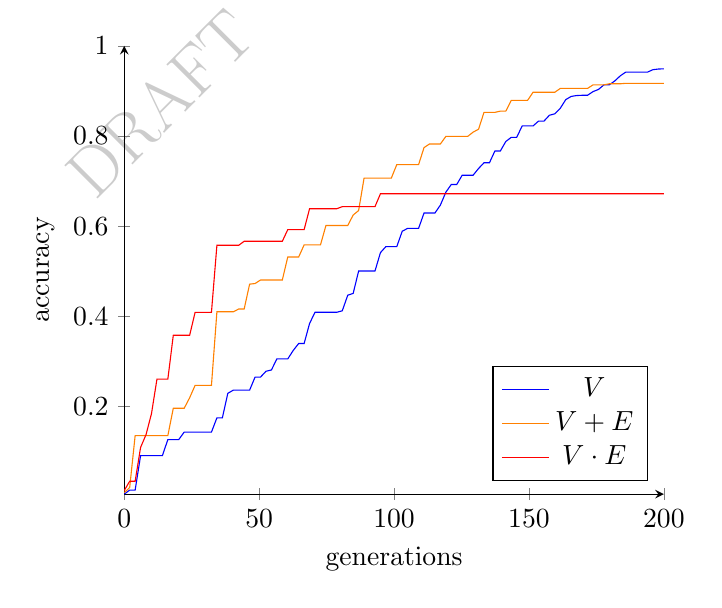
\begin{tikzpicture}
        \begin{axis}[
            axis lines = left,
            xlabel = generations,
            ylabel = accuracy,
            legend pos=south east,
            ymax=1
        ]
       \legend{$V$,$V+E$,$V\cdot E$}
            
        \addplot[color=blue]
        coordinates{(0, 0.0057)(2.020202e+00, 0.0147)(4.040404e+00, 0.0147)(6.060606e+00, 0.0912)(8.080808e+00, 0.0912)(1.010101e+01, 0.0912)(1.212121e+01, 0.0912)(1.414141e+01, 0.0912)(1.616162e+01, 0.1267)(1.818182e+01, 0.1267)(2.020202e+01, 0.1267)(2.222222e+01, 0.1433)(2.424242e+01, 0.1433)(2.626263e+01, 0.1433)(2.828283e+01, 0.1433)(3.030303e+01, 0.1433)(3.232323e+01, 0.1433)(3.434343e+01, 0.1749)(3.636364e+01, 0.1749)(3.838384e+01, 0.2293)(4.040404e+01, 0.2363)(4.242424e+01, 0.2363)(4.444444e+01, 0.2363)(4.646465e+01, 0.2363)(4.848485e+01, 0.2653)(5.050505e+01, 0.2653)(5.252525e+01, 0.2782)(5.454545e+01, 0.2811)(5.656566e+01, 0.3056)(5.858586e+01, 0.3056)(6.060606e+01, 0.3056)(6.262626e+01, 0.3244)(6.464646e+01, 0.3397)(6.666667e+01, 0.3397)(6.868687e+01, 0.3842)(7.070707e+01, 0.4091)(7.272727e+01, 0.4091)(7.474747e+01, 0.4091)(7.676768e+01, 0.4091)(7.878788e+01, 0.4091)(8.080808e+01, 0.4123)(8.282828e+01, 0.4468)(8.484848e+01, 0.4510)(8.686869e+01, 0.5005)(8.888889e+01, 0.5005)(9.090909e+01, 0.5005)(9.292929e+01, 0.5005)(9.494949e+01, 0.5413)(9.696970e+01, 0.5547)(9.898990e+01, 0.5547)(1.010101e+02, 0.5547)(1.030303e+02, 0.5888)(1.050505e+02, 0.5952)(1.070707e+02, 0.5952)(1.090909e+02, 0.5952)(1.111111e+02, 0.6292)(1.131313e+02, 0.6292)(1.151515e+02, 0.6292)(1.171717e+02, 0.6468)(1.191919e+02, 0.6753)(1.212121e+02, 0.6925)(1.232323e+02, 0.6925)(1.252525e+02, 0.7130)(1.272727e+02, 0.7130)(1.292929e+02, 0.7130)(1.313131e+02, 0.7279)(1.333333e+02, 0.7406)(1.353535e+02, 0.7406)(1.373737e+02, 0.7668)(1.393939e+02, 0.7668)(1.414141e+02, 0.7878)(1.434343e+02, 0.7970)(1.454545e+02, 0.7970)(1.474747e+02, 0.8223)(1.494949e+02, 0.8223)(1.515152e+02, 0.8223)(1.535354e+02, 0.8330)(1.555556e+02, 0.8330)(1.575758e+02, 0.8460)(1.595960e+02, 0.8492)(1.616162e+02, 0.8616)(1.636364e+02, 0.8807)(1.656566e+02, 0.8878)(1.676768e+02, 0.8897)(1.696970e+02, 0.8903)(1.717172e+02, 0.8903)(1.737374e+02, 0.8984)(1.757576e+02, 0.9032)(1.777778e+02, 0.9134)(1.797980e+02, 0.9136)(1.818182e+02, 0.9222)(1.838384e+02, 0.9334)(1.858586e+02, 0.9417)(1.878788e+02, 0.9417)(1.898990e+02, 0.9417)(1.919192e+02, 0.9417)(1.939394e+02, 0.9417)(1.959596e+02, 0.9471)(1.979798e+02, 0.9485)(200, 0.9490)};

        \addplot[color=orange]
        coordinates{(0, 0.0090)(2.020202e+00, 0.0204)(4.040404e+00, 0.1355)(6.060606e+00, 0.1355)(8.080808e+00, 0.1355)(1.010101e+01, 0.1355)(1.212121e+01, 0.1355)(1.414141e+01, 0.1355)(1.616162e+01, 0.1355)(1.818182e+01, 0.1962)(2.020202e+01, 0.1962)(2.222222e+01, 0.1962)(2.424242e+01, 0.2195)(2.626263e+01, 0.2469)(2.828283e+01, 0.2469)(3.030303e+01, 0.2469)(3.232323e+01, 0.2469)(3.434343e+01, 0.4101)(3.636364e+01, 0.4101)(3.838384e+01, 0.4101)(4.040404e+01, 0.4101)(4.242424e+01, 0.4163)(4.444444e+01, 0.4163)(4.646465e+01, 0.4714)(4.848485e+01, 0.4728)(5.050505e+01, 0.4806)(5.252525e+01, 0.4806)(5.454545e+01, 0.4806)(5.656566e+01, 0.4806)(5.858586e+01, 0.4806)(6.060606e+01, 0.5317)(6.262626e+01, 0.5317)(6.464646e+01, 0.5317)(6.666667e+01, 0.5584)(6.868687e+01, 0.5584)(7.070707e+01, 0.5584)(7.272727e+01, 0.5584)(7.474747e+01, 0.6014)(7.676768e+01, 0.6014)(7.878788e+01, 0.6014)(8.080808e+01, 0.6014)(8.282828e+01, 0.6014)(8.484848e+01, 0.6247)(8.686869e+01, 0.6347)(8.888889e+01, 0.7067)(9.090909e+01, 0.7067)(9.292929e+01, 0.7067)(9.494949e+01, 0.7067)(9.696970e+01, 0.7067)(9.898990e+01, 0.7067)(1.010101e+02, 0.7366)(1.030303e+02, 0.7366)(1.050505e+02, 0.7366)(1.070707e+02, 0.7366)(1.090909e+02, 0.7366)(1.111111e+02, 0.7743)(1.131313e+02, 0.7823)(1.151515e+02, 0.7823)(1.171717e+02, 0.7823)(1.191919e+02, 0.7990)(1.212121e+02, 0.7990)(1.232323e+02, 0.7990)(1.252525e+02, 0.7990)(1.272727e+02, 0.7990)(1.292929e+02, 0.8085)(1.313131e+02, 0.8150)(1.333333e+02, 0.8524)(1.353535e+02, 0.8524)(1.373737e+02, 0.8524)(1.393939e+02, 0.8551)(1.414141e+02, 0.8551)(1.434343e+02, 0.8791)(1.454545e+02, 0.8791)(1.474747e+02, 0.8791)(1.494949e+02, 0.8791)(1.515152e+02, 0.8970)(1.535354e+02, 0.8970)(1.555556e+02, 0.8970)(1.575758e+02, 0.8970)(1.595960e+02, 0.8971)(1.616162e+02, 0.9055)(1.636364e+02, 0.9055)(1.656566e+02, 0.9055)(1.676768e+02, 0.9055)(1.696970e+02, 0.9055)(1.717172e+02, 0.9055)(1.737374e+02, 0.9134)(1.757576e+02, 0.9134)(1.777778e+02, 0.9134)(1.797980e+02, 0.9158)(1.818182e+02, 0.9158)(1.838384e+02, 0.9158)(1.858586e+02, 0.9168)(1.878788e+02, 0.9168)(1.898990e+02, 0.9168)(1.919192e+02, 0.9168)(1.939394e+02, 0.9168)(1.959596e+02, 0.9168)(1.979798e+02, 0.9168)(200, 0.9168)};

        \addplot[color=red]
        coordinates{(0, 0.0137)(2.020202e+00, 0.0343)(4.040404e+00, 0.0343)(6.060606e+00, 0.1094)(8.080808e+00, 0.1377)(1.010101e+01, 0.1843)(1.212121e+01, 0.2607)(1.414141e+01, 0.2607)(1.616162e+01, 0.2607)(1.818182e+01, 0.3581)(2.020202e+01, 0.3581)(2.222222e+01, 0.3581)(2.424242e+01, 0.3581)(2.626263e+01, 0.4089)(2.828283e+01, 0.4089)(3.030303e+01, 0.4089)(3.232323e+01, 0.4089)(3.434343e+01, 0.5576)(3.636364e+01, 0.5576)(3.838384e+01, 0.5576)(4.040404e+01, 0.5576)(4.242424e+01, 0.5576)(4.444444e+01, 0.5665)(4.646465e+01, 0.5665)(4.848485e+01, 0.5665)(5.050505e+01, 0.5665)(5.252525e+01, 0.5665)(5.454545e+01, 0.5665)(5.656566e+01, 0.5665)(5.858586e+01, 0.5665)(6.060606e+01, 0.5923)(6.262626e+01, 0.5923)(6.464646e+01, 0.5923)(6.666667e+01, 0.5923)(6.868687e+01, 0.6387)(7.070707e+01, 0.6387)(7.272727e+01, 0.6387)(7.474747e+01, 0.6387)(7.676768e+01, 0.6387)(7.878788e+01, 0.6387)(8.080808e+01, 0.6433)(8.282828e+01, 0.6433)(8.484848e+01, 0.6433)(8.686869e+01, 0.6433)(8.888889e+01, 0.6433)(9.090909e+01, 0.6433)(9.292929e+01, 0.6433)(9.494949e+01, 0.6718)(9.696970e+01, 0.6718)(9.898990e+01, 0.6718)(1.010101e+02, 0.6718)(1.030303e+02, 0.6718)(1.050505e+02, 0.6718)(1.070707e+02, 0.6718)(1.090909e+02, 0.6718)(1.111111e+02, 0.6718)(1.131313e+02, 0.6718)(1.151515e+02, 0.6718)(1.171717e+02, 0.6718)(1.191919e+02, 0.6718)(1.212121e+02, 0.6718)(1.232323e+02, 0.6718)(1.252525e+02, 0.6718)(1.272727e+02, 0.6718)(1.292929e+02, 0.6718)(1.313131e+02, 0.6718)(1.333333e+02, 0.6718)(1.353535e+02, 0.6718)(1.373737e+02, 0.6718)(1.393939e+02, 0.6718)(1.414141e+02, 0.6718)(1.434343e+02, 0.6718)(1.454545e+02, 0.6718)(1.474747e+02, 0.6718)(1.494949e+02, 0.6718)(1.515152e+02, 0.6718)(1.535354e+02, 0.6718)(1.555556e+02, 0.6718)(1.575758e+02, 0.6718)(1.595960e+02, 0.6718)(1.616162e+02, 0.6718)(1.636364e+02, 0.6718)(1.656566e+02, 0.6718)(1.676768e+02, 0.6718)(1.696970e+02, 0.6718)(1.717172e+02, 0.6718)(1.737374e+02, 0.6718)(1.757576e+02, 0.6718)(1.777778e+02, 0.6718)(1.797980e+02, 0.6718)(1.818182e+02, 0.6718)(1.838384e+02, 0.6718)(1.858586e+02, 0.6718)(1.878788e+02, 0.6718)(1.898990e+02, 0.6718)(1.919192e+02, 0.6718)(1.939394e+02, 0.6718)(1.959596e+02, 0.6718)(1.979798e+02, 0.6718)(200, 0.6718)};
        \end{axis}
    \end{tikzpicture}
              \caption{A comparison of the accuracy of networks with different formulae determining the number of \eqprop iterations per generation. The task used for testing was the classification of Iris flowers into three classes: setosa, versicolor and virginica. }
              \label{fig:network_com_iter}
          \end{figure}
        
  
		\subsection{Hardware acceleration}
		As mentioned in the introduction, \eqprop was designed with effective hardware implementations in mind. It has been shown \cite{hardware_eq}, that the \eqprop training of purely analog neural networks is indeed, possible. The missing piece for accelerating most of the EqPropNEAT stages is the capability to dynamically create the analog neural network representations for the current population. This would allow the use of hardware implemented \eqprop for high-speed training. 
		
		Fortunately, field-programmable analog arrays (FPAA) provide an off-the-shelf solution for reprogramming the interconnects between different analog devices, enabling the creation of hardware based analog neural networks \cite{fpaa-neural-network} while our algorithm is running. However, implementing \eqprop requires the ability to efficiently measure voltages in our network, as well as additional circuitry for digital operations such as computing the gradient. Field-programmable gate arrays (FPGA) are a much more popular digital counterpart to FPAAs. For our use case, a mixture of both systems is needed. While such devices have been already proposed in technical literature \cite{fgbfpmsa}, to the best of our knowledge, they have never been manufactured in a meaningful quantity yet. In theory, a mostly hardware accelerated implementation of our algorithm will be possible, once the above mentioned hardware becomes widely available. Figure \ref{fig:hardware} shows an outline of this algorithm. 
		
		Although at first glance the proposed hardware acceleration seems to improve runtimes significantly, we must mention a couple of potential performance limiting bottlenecks. Genetic algorithms in general require a population with thousands of genoms to provide enough diversity. Without this the algorithm does not work, or at least needs a lot more generations to arrive at a solution. It is also even more susceptible to overfitting. However with thousands of neural networks, with each of them potentially having at least hundreds of nodes, the required circuitry becomes problematically large. There is a high chance that even if the required hardware becomes available, it probably will only be able to contain a fraction of the population at a time. Of course this problem can be somewhat alleviated by splitting the population into groups which are evaluated and trained in separate passes (yielding slower runtime), however this way the number of occasions when the FPMA hardware is reconfigured with the new networks grows. In the case of modern day FPGAs the time it takes to reconfigure the entire board is usually in the realm of seconds, although by sacrificing some parts of the board for as a cache, this can be dramatically improved \cite{runtime-partial-reconfiguration-speed}. In any case it is best to avoid reconfiguration as much as possible. At the time of writing this paper it is impossible to tell how much of a limiting factor this will be.
		
		Another potential issue is the lifetime of the hypothetic hardware as many frequent reconfigurations might degrade the board significantly. Runtime partial reconfiguration can also be employed to correct appearing hardware errors as the board ages \cite{runtime-partial-reconfiguration-reliability}. Unfortunately this comes at a cost of reduced usable board area and as a result, a smaller limit on the number of neural networks we can evaluate in parallel.  %Nowadays a typical FPGA 
		
		%TODO: slow reconfiguration, hardware lifetime, runtime partial reconfiguration
		\tikzstyle{cloud} = [rectangle, draw, fill=gray!20, text width=1cm, text centered, minimum height=1.5em, rounded corners]
		\begin{figure}
			\centering
			\begin{tikzpicture}[node distance = 1.5cm, auto]
				\node[cloud, text width=4cm](init){Initialize population and create analog networks on FPMA};
				\node[cloud, text width=4cm, below of=init](eval){Evaluate the genomes (in hardware)};
				\node[cloud, text width=4cm, below of=eval](fromfpma){Copy results back from FPMA};
				\node[cloud, text width=2cm, below of=fromfpma](cross){Crossover};
				\node[cloud, text width=4cm, below of=cross](mut){Mutations without random edge weight changing rule};
				\node[cloud, text width=4cm, below of=mut](tofpma2){Create analog networks on FPMA};
				\node[cloud, text width=4cm, below of=tofpma2](eqprop){Equilibrium propagation iterations (in hardware)};
				
				\coordinate (A) at ($(eval.east)+(1cm,0cm)$);
				\coordinate (B) at ($(eqprop.east)+(1cm,0cm)$);
				
				\draw[->, arrows = {-{Stealth[scale=1.5]}}](init)--(eval);
				%\draw[->, arrows = {-{Stealth[scale=1.5]}}](tofpma1)--(eval);
				\draw[->, arrows = {-{Stealth[scale=1.5]}}](eval)--(fromfpma);
				\draw[->, arrows = {-{Stealth[scale=1.5]}}](fromfpma)--(cross);
				\draw[->, arrows = {-{Stealth[scale=1.5]}}](cross)--(mut);
				\draw[->, arrows = {-{Stealth[scale=1.5]}}](mut)--(tofpma2);
				\draw[->, arrows = {-{Stealth[scale=1.5]}}](tofpma2)--(eqprop);
				\draw[->, arrows = {-{Stealth[scale=1.5]}}] (eqprop) -- (B) -- node [right, align=left] {Repeat until good enough\\ solution is found} (A) -- (eval);
			\end{tikzpicture}
			\caption{An outline of the hardware accelerated EqPropNEAT algorithm. Note that the evaluation and weight training of genomes is entirely accomplished on the hardware level.}
			\label{fig:hardware}
		\end{figure}
		\subsection{Biologically plausible algorithm}
		One of the goals of this study is the creation of a biologically plausible neural network model. For the generation of the network we went with a well tested solution, namely: NEAT. For the fine tuning of weights the obvious solution would have been the BP which offers great performance and is well tested and widely used to solve various task. However because of the aforementioned criteria of having a biologically plausible algorithm BP is off the table. For this reason we choose EP which utilizes a very similar concept with one key difference: it is considered biologically plausible. The fact that EP uses the same algorithm for both phases of training from one perspective made the hardware acceleration possible, but looking at it from another direction we can see that this  also makes it a biologically plausible solution. Knowing this it's easy to see why BP's usage of different algorithms for these phases leads to the fact that it is considered biologically implausible. This way it's possible for the model to accurately represent the neural network of a living creature.
		
		Of course this whole idea only makes sense if the performance remains at similar levels to those of conventional solutions. In general the performance of EP is subpar compared to BP due the unique restriction of only using one algorithm for both training phases. This problem can be mitigated by the aforementioned hardware acceleration technique. We will discuss the results further in the \textit{Performance} chapter. As we have proven the performance can be a match or even an improvement compared to contemporary solutions thus we are left with only the benefits and no downsides. Benefits being the reduced complexity due to only one function being used for training and as a consequence of this the biological plausibility.
		
		Considering the results and implications of EqPropNeat we should be able to accurately reconstruct a living creature's neural network and with the proper hyperparameters. In theory we would be able to create a neural network which would engage the neurons in the same place and in the same order as the biological network it was based on. This would get us as closer to understanding how the brain works and also would raise some ethical questions but that is beyond the scope of this paper and this is only in theory so far.
		\section{Results}
        \subsection{Performance}
        We evaluated our method on several benchmarks, which are commonly used for comparison of neuroevolution techniques. Comparison was made with the NEAT implementation of the original author (K. Stanley) \cite{neatcpp} and a self made implementation of the Learning-NEAT method \cite{lneat} (as the original authors did not share their implementation). Tha latter is particularly important, since our method is mostly derived from Learning-NEAT, by substituting backpropagation with equilibrium propagation.

        One of the benchmarks was classic pole balancing. In this problem, the neural network has to keep a pole balanced for a given amount of time.

        \begin{figure}
            \centering
            \begin{tabular}{|l||c|c|c|}
            \hline
           & NEAT & EqPropNEAT & Learning-NEAT \\
                \hline\hline
               Successful & 3& 10& 12\\\hline
               Failed & 17& 10 & 8 \\\hline
               Success rate & 15\% & 50\% & 60\%\\\hline
            \end{tabular}
            \caption{Success rates of the different NEAT derived techniques at the 2D pole balancing task. An attempt was deemed successful if the network managed to keep the pole balanced over 6000 simulation steps (10 seconds). All methods were run 20 times, the percentages tell the ratio of successful runs where the algorithm managed to train a network that could solve the problem.}
            \label{fig:rates-2dpole}
        \end{figure}

        Another benchmark was the 2D pole balancing task \cite{pole2d}. This is a harder version of the classic pole balancing problem, in which the pole is balanced on top of a movable 2D plane, instead of a line segment. Figure \ref{fig:rates-2dpole} shows the success rates of the tested methods. Note that our method fares batter than the original NEAT algorithm, however it falls a bit short of Learning-NEAT. The reason for this is that due to the poor runtime of software \eqprop, we had to use less \eqprop iterations than ideal. For this task we used feed-forward neural networks, which is the reason why the results are worse then in \cite{pole2d} where recurrent networks were used. 
    
        \begin{figure}
            \centering
            \begin{tabular}{|l||c|c|c|}
            \hline
           & NEAT & EqPropNEAT & Learning-NEAT \\
                \hline\hline
               Successful & 3& 10& 12\\\hline
               Failed & 17& 10 & 8 \\\hline
               Success rate & 15\% & 50\% & 60\%\\\hline
            \end{tabular}
            \caption{Success rates of the different NEAT derived techniques at the 2D pole balancing task. An attempt was deemed successful if the network managed to keep the pole balanced over 6000 simulation steps (10 seconds). All methods were run 20 times, the percentages tell the ratio of successful runs where the algorithm managed to train a network that could solve the problem.}
            \label{fig:rates-2dpole}
        \end{figure}

    

        \section{Discussion and conclusion}
		After conducting our experiments we can positively say that the proposed method performs up to expectations in the accuracy front and it can achieve similar performance to the contemporary algorithms. In terms of learning speeds of course it is currently behind the cutting edge without the specialized hardware. Despite this simulations indicate that with the aforementioned special hardware the EqPropNEAT algorithm can far outperform current rivals in terms of learning speed. This would present new possibilities for applications of AI. The speed of learning and predicting based on simulations could be close to real time, which would mean that with the proper hardware we could have individual devices learning separately without using a centralised dataset or an already created and weight adjusted neural network. 
		%\begin{thebibliography}{1}
		\bibliographystyle{IEEEtran}
		\bibliography{references}
		
		%  \end{thebibliography}
	
\end{document}
